\chapter{Small Sphere Experiment}
\label{chap:SmallSphere}

\textit{The work presented here has been presented as an invited oral presentation by Lindsay MacDonald at AIC 2017 \citep{macdonald_melanopsin_2017}\footnote{The proceedings are not yet available, though a note at \url{https://aic-color.org/page-18077} suggests that they will soon be available.}.}


\section{Summary}

Ethics: \dots
Code and data are provided: \url{https://github.com/da5nsy/Small-Sphere}.

\section{Introduction}

% why this experiment? Response to issues in large sphere
% - luminance
% - too many variables
% research question

This experiment was performed to develop upon the Large Sphere experiment by narrowing down the number of variables and more directly testing the hypothesis that melanopsin is involved in colour constancy. This was achieved using a similar experimental set-up to the previous experiment, with several key alterations:

\begin{enumerate}
    \item Instead of 16 surround conditions, only two were included.
    \begin{enumerate}
        \item These two conditions were designed to be perceptual metamers for each observer, but with maximally different levels of melanopic activation.
    \end{enumerate}
    \item Instead of 16 lightness conditions, only 5 were included.
    \item The sphere used was smaller, and painted with a higher reflectance paint, with the hope of increasing the level of adapting radiation.
    \item Three observers were tested (the author and two colleagues of a similar age), with multiple repeats of each condition.
\end{enumerate}

Further details on all of the above amendments will be included in the following sections. 

The null hypothesis that this experiment aims to test is that melanopsin activation does not alter an observers perceptual white point.

\section{Materials and Methods}

\subsection{Hardware}

The sphere used in this experiment was roughly 400mm in diameter, with ports of similar functions to those which were present in the Large Sphere. On one side there is a padded port for an observer's face. Mirroring this is a small aperture through which an LCD screen is visible. At the top of the sphere was a port through which illumination was provided. An additional port, on the observer's side of the base, was added such that the illumination provided to the sphere could be unobtrusively monitored throughout experiments.

\begin{figure}[htbp]
%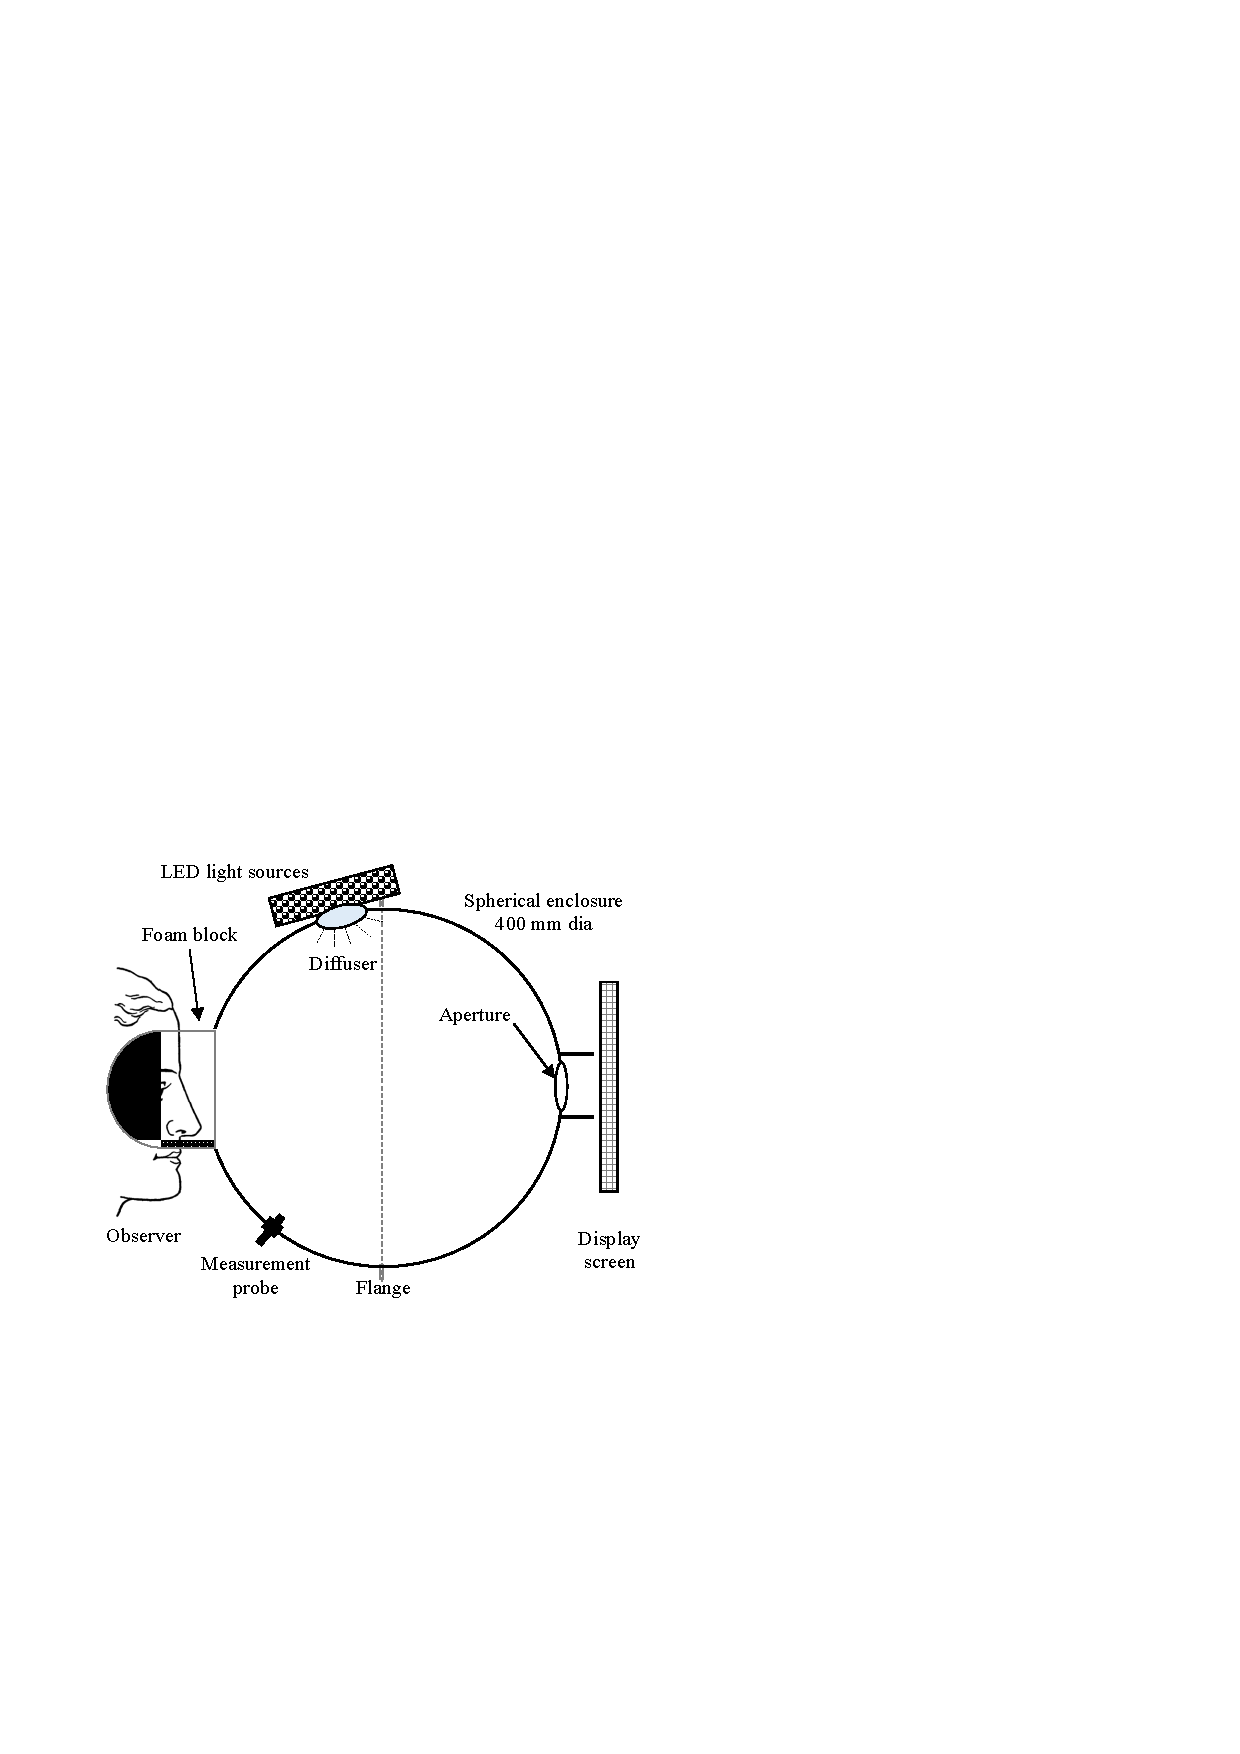
\includegraphics[max width=\textwidth,center]{figs/SmallSphere/diagram.pdf}
\caption{The small sphere set up, reproduced from \citet{macdonald_melanopsin_2017}, courtesy of Lindsay MacDonald.}
\label{fig:diagram}
\end{figure}

\subsection{The sphere}

% diagram 
% photo

The sphere used in this experiment was somewhat smaller than the one used in the previous experiments (hence the experiment short-hand names) and this served several purposes. 

The illumination in the Large Sphere had been rather low, partly such that rod interactions would be made visible, and partly due to practical limitations. The grey paint on the interior of the Large Sphere was chosen such to limit specular reflections, but it meant that overall illumination levels were very low. In the small sphere, it was hoped that my reducing the size of the sphere that it might be possible to keep the illumination slightly higher, as it would be spread across a smaller surface. Additionally, of practical concern, it was easier to find experimental space for a smaller sphere.

Several paints were trialled for use in the small sphere. The required conditions were that they were available as a spray, and provided as `matt white'. Sample patched were sprayed to assess finish and spectral reflectance. It was seen as beneficial if: the finish had a very fine grain and as little gloss to it as possible, the surface reflectance was high and the \gls{SRF} was an uniform across the spectrum as possible. It was also considered a requisite requirement that any paint should not include any fluorescent whitening agents (such as can be seen in the `white paper' data shown in Figure \ref{fig:spray}).

Measurements of the \glspl{SRF} of the 8 tested spray-paints, and further details of the spray-paints themselves, can be seen in Figure \ref{fig:spray}. It can be seen that Montana Gold Sh. White Cream and Pebble, along with MTN 94 RV-198 are either too low in reflectance, or not spectrally uniform enough. The two with the most desirable finishes were the Flame Blue and MTN Water Based paints. The MTN Water Based paint was chosen due to its particularly fine-grain finish.

\begin{figure}[htbp]
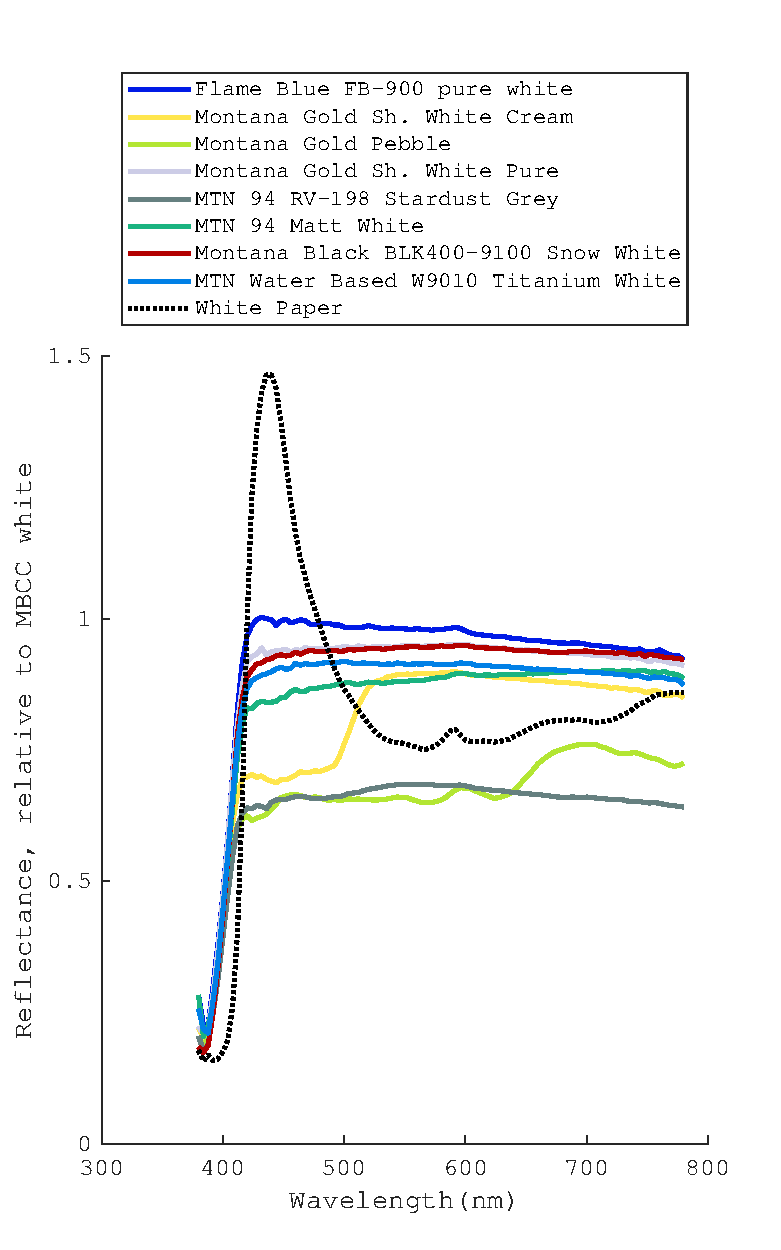
\includegraphics[max width=1.2\textwidth,center]{figs/SmallSphere/VisualiseSPDs_result.pdf}
\caption{The \glspl{SRF} of the 8 tested paints (relative to the white patch of a MacBeth Colour Checker card, which is known to be very uniform in spectral reflectance) with an additional measurement of a piece of white office paper to demonstrate how a fluorescent additive might appear. Data available: \url{https://github.com/da5nsy/Small-Sphere/tree/master/Hardware\%20Specs/WhiteSprayPaints}}
\label{fig:spray}
\end{figure}


\subsection{The screen}

The screen was offset by roughly 150mm through a short black paper tube in order to limit the interference (either way) between the screen illuminant and the sphere illuminant. 

%Primaries
%Gamut

\subsubsection{Characterisation}

Following the disappointment of the data collection phase of the Large Sphere experiment, two separate characterisation procedures were performed, one before and one after every set of observations (in addition to the monitoring of illumination inside the sphere).

The first characterisation routine is rather standard - a spectral measurement of the display primaries followed by a ramping through pixel space for each display channel from zero output to maximum output\footnote{Controlled by the script available at \url{https://github.com/da5nsy/Small-Sphere/blob/5c6af38c5036a4c0a328a9854427ae8e851e84fd/Hardware\%20Specs/PR650\%20Screen\%20Measurements/PR650displaycharacterisation_DG.m}}. This was only measured for the small portion of the screen which would be used during experiments.

The second calibration procedure attempted to include any issues which may arise due to the specific specification method used within the experiment. A very minor amendment was made to a copy of the main experimental script, such that it only included 3 repeats rather than 30. %haven't introduced this yet
This script was run in exactly the same way that the main experimental script would be run, except that the observer was replaced by our \gls{PR650}, and no effort was made to select neutral points, with a measurement being made of each presentation. In this way, a random selection of points were recorded, and through comparison with the recorded `responses', it could be seen whether there was any discrepancy between what we thought was being displayed on the screen and what was actually being displayed on the screen.
% demo?

\subsection{The LED rig}

The lighting in this experiment was designed such that two lighting conditions could be defined for each observer which were perceptual metamers (in the periphery, at high temporal frequencies), but which differed in melanopic activation.

Four types of LED, to operate as two pairs, were chosen to maximise melanopic contrast between the pairs. An additional limitation was that no LED with a peak lower than 400nm was to be used (due to safety concerns).

50 LEDs, mounted in a breadboard, were controlled by an Arduini Uno. %photo?

\begin{itemize}
    \item 20: Bivar UV5TZ-400-15 (henceforth `UV')
    \item 10: Cree C503B-BCS-CV0Z0461 (henceforth `blue')
    \item 10: Cree C503B-AAS-CA0C0251-015 (henceforth `amber')
    \item 10: Cree C503B-RAS-CY0B0AA2 (henceforth `red')
\end{itemize}

%UNOPENED 
%810-6705 C503D-WAN-CCbEb151
%810-6636 C503B-AAN-CY0B0251
%810-0492 C503B-BCN-CV0Z0461

\begin{figure}[htbp]
%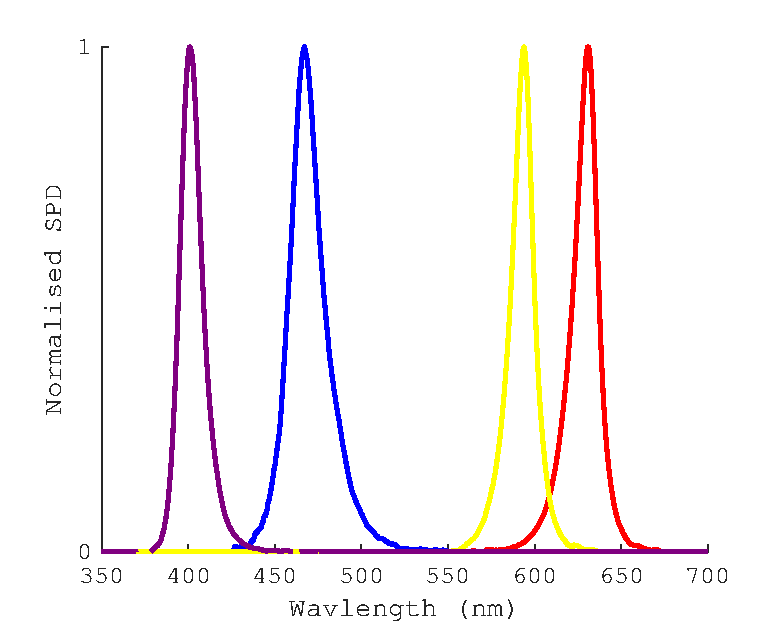
\includegraphics[max width=\textwidth,center]{figs/SmallSphere/LED_SPDs.pdf}
\caption{The normalised \glspl{SPD} of the Small Sphere \glspl{LED}.}
\label{fig:LED_SPDs}
\end{figure}

The arduino script set the \glspl{LED}, via pulse width modulation, to the output levels decided in the perceptual nulling segment of the experiment. The two modes had either the combination of UV and amber, or blue and red, allowing for the chromaticities falling upon the lines shown in Figure \ref{fig:LED_SPDs}. The combinations UV and blue, or amber and red, were never used.

\begin{figure}[htbp]
%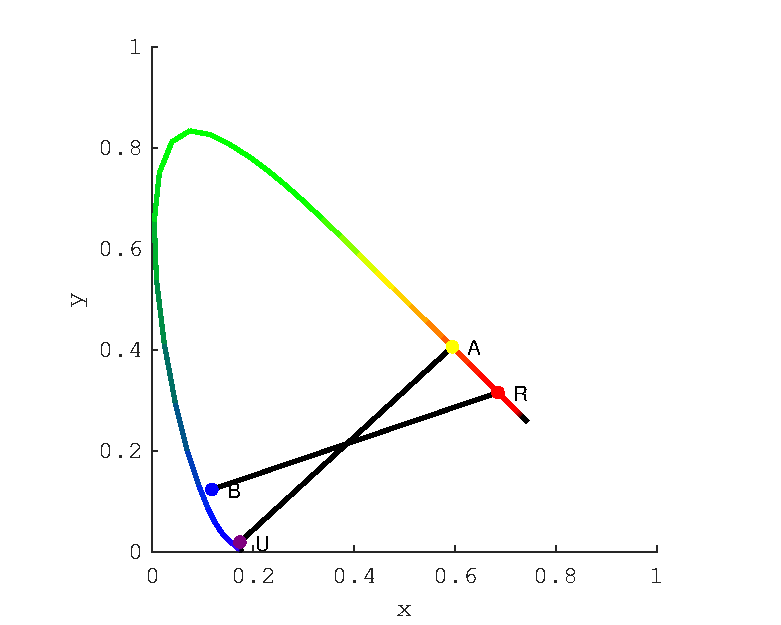
\includegraphics[max width=\textwidth,center]{figs/SmallSphere/LED_cross.pdf}
\caption{The chromaticities of the Small Sphere \glspl{LED} in CIE 1931 space.}
\label{fig:LED_cross}
\end{figure}

This breadboard was mounted stably atop the sphere with a perspex diffusion sheet between it and the opening into the sphere. Black card was used to mask stray light, mainly to address the specific concern that light may reach the LCD display.

Throughout the experiments the illumination inside the sphere was measured with an Ocean Optics USB 2000+ through a optical fiber probe mounted to the base of the sphere and directed at a point on the roof of the sphere, opposite the observer. It was expected that the output of the \glspl{LED} may change slightly over time. %fig x?

% safety
% The controllers 
% The code
% Characterisation / ongoing measurement

\subsection{Observer task}

\subsubsection{Perceptual Nulling}

The basic logic of this experiment is as follows: under the null hypothesis two adapting fields of identical appearance should adapt an observer in exactly the same way. In order to design two adapting field illuminants which appear identical (perceptual metamers) we can either make predictions based upon standard observers (with parameters set to match our real observers regards age and pupil dilation etc.) or we can provide a process whereby individual observers make minor alterations to the two conditions until they appear identical. We have opted to use colorimetry as a starting point to choose primaries, and then allow observers to fine-tune this matching.\footnote{A similar process to this has recently been used very effectively by \citet{allen_form_2019}.}

We run the risk of falling into circularity here: we ask observers to set two fields such that they appear identical, and then (in a roundabout way) we ask them whether there is any visual difference between them. If melanopsin does have a direct impact upon visual perception we are at risk of accounting for this at this stage.

Attempting to avoid this problem, we perform the perceptual nulling under conditions which we predict should not allow for \gls{ipRGC} involvement, or should minimise such. It seems to be the case that \glspl{ipRGC} do not react strongly over very short timescales ($<$0.5hz \citep{spitschan_human_2017-1}), with cones being much more active in this temporal window, so we chose to rapidly alternate between the two conditions and ask observers to make alterations until there is a minimal visible flicker.

Observers were instructed to fixate upon a small fixation point displayed at the centre of the otherwise dark display. They placed their hands upon three dials which could be independently varied to change the peripheral adapting illuminant inside the sphere.

Two modes were presented to observers, one where the two conditions were presented at 30hz for 1 second, followed by a 10 second break, and one where the conditions were presented at 4hz for 500ms, followed by a 1 second break. 

During the first condition the observer was requested only to alter the setting of the first dial, which would alter the overall level of the red/blue combination (whilst the uv/amber combination kept the same level).

During the second condition the observer was requested only to alter the settings of the second and third dial. The second dial would alter the relative contributions of red/blue to the first condition. The third dial would alter the relative contributions of uv/amber to the second condition. These options can be thought of as traversing the straight lines in Figure \ref{fig:LED_cross}.

The observer was allowed to switch back and forth between these two modes until they were happy with the match. Observers found this task rather difficult, predominantly due to the inherent difficulty in making colour matches in the periphery. An additional difficulty was that since eye movements were not strictly controlled, if an observer were to briefly look away from the fixation they would be able to see the adapting field with their foveal vision. This was problematic since in most cases the peripheral matches induced strong contrast for foveal perception. Though it was unintentional, this seems to be a particularly effective way of generating the perception of a Maxwell spot.

Despite these difficulties, observers generally found settings which for them resulted in a metameric match (where they could no longer perceive flicker). One observer who initially agreed to be part of the study withdrew at this stage, partly due to a difficulty completing this task, but mainly due to a claustrophobic nature. Another potential observer withdrew at this stage, since they were unable to make a match using this set of primaries, which we attribute to incipient cataracts.

This method has since been improved upon by \citet{allen_form_2019} who used a 2AFC task instead of a method of manual adjustment to pinpoint areas of perceptual metamerism.

% Observers were...
% Initial metamer setting
% Achromatic selections

\section{Results}


\section{Discussion}
% Assumptions
